\documentclass[11pt, a4paper]{report}

\usepackage{fullpage}
% A more tightly packed list than the standard
% \enumerate{itemize} append * after enumeration type
\usepackage{mdwlist}
% Multi-page tables + accompanying header and footer comments
\usepackage{longtable}

% Vertical table headers, not sure what does what. graphicx is
% multi-purpose and does a lot of other stuff like including images
\usepackage{array,graphicx}
\usepackage{booktabs}

% Lossless .png format expected for figures
\DeclareGraphicsExtensions{.png}

% \verbatiminput command (\begin{verbatim} is standard lib)
% This is used to include sql code from a .sql file
\usepackage{verbatim}

% `\rot{text}' is used to rotate 'text' by 90 degrees. To be used
% in tables where vertical column labeling is preferred.
\newcommand*\rot{\rotatebox{90}}


\title{Modeling a Blah Enterprise}
\author{John Appleseed\\ Loyola Marymount University\\ Database Systems}

% Allow commands
\providecommand\phantomsection{}

% Custom ToC labeling
\renewcommand\thechapter{\Roman{chapter}}
\renewcommand\thesection{\thechapter.\arabic{section}}

% Custom ToC spacing between chapter number and
% chapter name
\usepackage{tocloft}
\setlength{\cftchapnumwidth}{3em}
\setlength{\cftsecnumwidth}{3.5em}
\setlength{\cftsubsecnumwidth}{4em}

\begin{document}

%---    Title page    ---%
\clearpage
\phantomsection
\addcontentsline{toc}{chapter}{%
    \protect\numberline{I}Title Page}
\maketitle

%---    ToC    ---%
\clearpage
\phantomsection
\addcontentsline{toc}{chapter}{%
    \protect\numberline{II}Contents}
\tableofcontents
% The title page and ToC are difficult to handle,
% we set the page and chapter counter after the
% ToC is generated so that the rest of the document
% can continue on from there.
\setcounter{page}{2}
\setcounter{chapter}{2}

%---    Description of the Enterprise    ---%
\chapter{Description of the Enterprise}


\clearpage
\section{Ten Sample Questions}
\begin{enumerate}
    \item First question
    \item Second question
    \item Third question
\end{enumerate}

%---    Definition of Environment    ---%
\chapter{Definition of Environment}

\section{Input and Report forms}

% Number forms
\begin{enumerate}
\item Blah-blah View
    % itemize* is a more compacted list, imported by mdwlist
  \begin{itemize*}
    \item Blah name
    \item Blah url
    \item Total number of blah's
    \item Date created
  \end{itemize*}
 
\end{enumerate}

\clearpage
\section{Assumptions}
\begin{enumerate}
\item First good assumption
\item Another good assumption
\end{enumerate}

\clearpage
\section{User-oriented data dictionary}

% `p{<width>}` instread of `l` allows for multi-line text within a cell
% because it fixes the width of the cell rather than stretching to the longest element
\begin{longtable}{|l|p{10cm}|}

\hline
\textbf{Datum} & \textbf{Information Definition} \\ \hline

blah\_email    & Email of a Blah                 \\ \hline

\end{longtable}


\clearpage
\section{Cross-reference table}

% Here I include a couple lines of my 11 column Cross-reference table
% Try to see the patterns of what is going on here and modify for your own work
\begin{longtable}{|l|l|l|l|l|l|l|l|l|l|l|}

\hline
\multicolumn{1}{|c|}{Datum} &
\multicolumn{10}{c|}{Form or Screen} \\[1ex]

\hline
                                   &   % empty label block
\rot{Video Metadata View}          &
\rot{Song Metadata View}           &
\rot{Add New Physical good}        &
\rot{Add New Digital good}         &
\rot{Physical Good Admin}          &
\rot{Digital Good Admin}           &
\rot{Physical Consumer Admin View} &
\rot{Digital Consumer Admin View}  &
\rot{Transaction Log}              &
\rot{Interaction Log} \\
\hline

c\_email                &   &   &   &   &   &   & x & x &   &   \\ \hline
c\_first\_name          &   &   &   &   &   &   & x & x &   &   \\ \hline


\end{longtable}

%---    Enterprise Database Design    ---%
\chapter{Enterprise Database Design}

\section{Logical model of the Enterprise}

\subsection{List of Entities and Attributes}


\clearpage
\subsection{List of Relationships and Attributes}


\clearpage
\subsection{Entity-Relationship diagram of the Enterprise}
% Uncomment the below line and replace `ERB.png' with the file name of your ERB diagram.
% The ERB should be in .png format and should be in the same directory as this .tex file
% 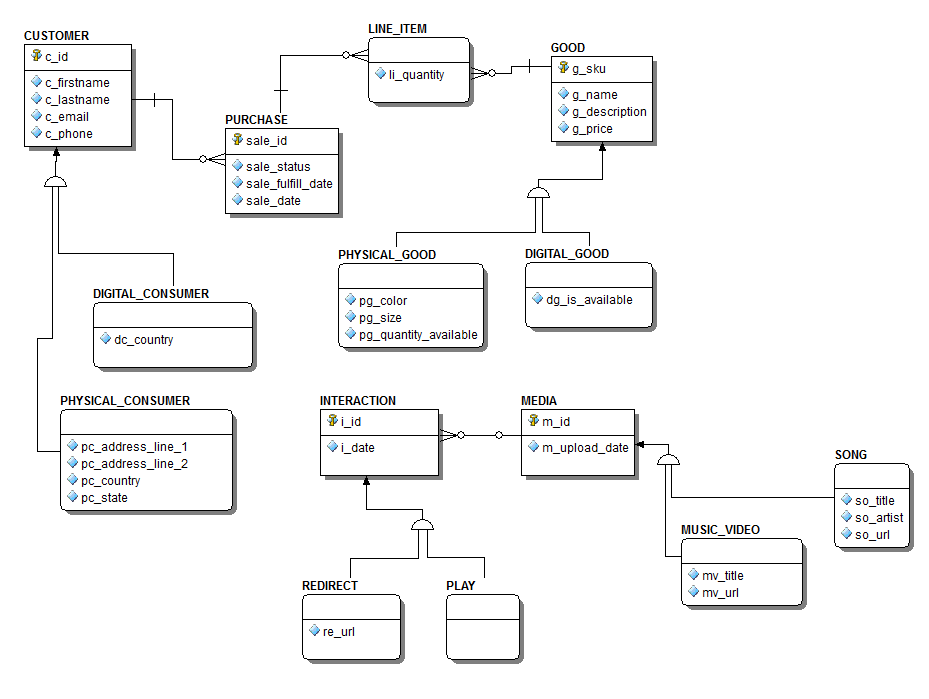
\includegraphics[width=\textwidth]{ERB.png}

\clearpage
\section{Conceptual model of the enterprise}


\clearpage
\section{Table dictionary}

% `p{<width>}` instread of `l` allows for multi-line text within a cell
% because it fixes the width of the cell rather than stretching to the longest element
\begin{longtable}{|l|p{4cm}|p{7cm}|}
\hline
\textbf{Table}      & \textbf{Attributes}                                                          & \textbf{Description}                                   \\ \hline

CUSTOMER            & c\_id, c\_firstname, c\_lastname, c\_email, c\_phone                         & Basic customer information                             \\ \hline

\end{longtable}

\clearpage
\section{Attribute dictionary}

% `p{<width>}` instread of `l` allows for multi-line text within a cell
% because it fixes the width of the cell rather than stretching to the longest element
\begin{longtable}{|l|p{4.4cm}|p{7cm}|}

\hline
\textbf{Datum}      & \textbf{Appears in}    & \textbf{Information Definition} \\ \hline

c\_email            & CUSTOMER               & Email                           \\ \hline

\end{longtable}

%---    Database and Query Definition    ---%
\chapter{Database and Query Definition}

\section{Database Definition}
    % Uncomment and replace filename with the filename of your outputted database generation code
    % \verbatiminput{online-music-business.sql}

\clearpage
\section{Database Queries}
    % Uncomment and replace filename with the filename of your 10 sql queries
    % \verbatiminput{db-queries-10-questions.sql}

\clearpage
\section{Design Tradeoffs and Limitations}

%---    Database Integrity and Security    ---%
\chapter{Database Integrity and Security}

\section{Functional Dependencies}

\noindent\textbf{Media Dependencies}
\begin{enumerate}
\item \texttt{m\_id} $\longrightarrow$ \texttt{m\_upload\_date, so\_id, mv\_id}

\end{enumerate}

\clearpage
\section{Adjustments for Normalization}
    An explanation of the changes needed to normalize your database.

\clearpage
\section{Integrity and Security}
    A list (in English) of the integrity and security constraints which are to hold on your database.

%---    Implementation Notes    ---%
\chapter{Implementation Notes}

\clearpage
\section{Indices}
    A list of the indices used by your database, with a justification for each.

\clearpage
\section{Data}
    The data used to populate your database.

\clearpage
\section{Query Trace}
    A trace of the execution of each of your queries.

\clearpage
\section{Implementation Assessment}
    An assessment of how smoothly your implementation went

%---    Lessons Learned    ---%
\chapter{Lessons Learned}

\end{document}
